\chapter{Podobna dela}
Globoke nevronske mreže močno vplivajo na raziskave v računalniškem vidu in strojnem učenju, saj po zmogljivostnih testih premagujejo večino algoritmov, ki jih je razvil človek \cite{sunderhauf2018the}. Zavedati se moramo, da imajo kljub temu DNN pomankljivosti, zato velikokrat odpovejo v realističnem okolju~\cite{sunderhauf2018the}. Glavni poudarek, zakaj prihaja do razlik med zmogljivostnimi testi na podatkovnih bazah in realnim okoljem je, da se pri zmogljivostnih testih raziskovalci osredotočajo na evaluacijske statistike, ki povzemajo zmogljivost algoritmov \cite{sunderhauf2018the}. Kot je poudaril \citea{sunderhauf2018the}: ``Če statistika govori, da je bila podatkovna baza rešena, še ne pomeni, da je bil problem rešen." Trditve, da so nevronske mreže presegle človeško zmogljivost, temeljijo na zmogljivostnih testih in so napačne ter zavajujoče. Pri primerjanju zmogljivosti z ljudmi bi potrebovali drugačen pristop, kot je vizualna psihofizika, ki je predstavljena v nadaljevanju. 


Nadaljnje, podatkovne baze ne povzemajo naravnih scenarijov, saj so te zgrajene na slikah in video posnetkih iz interneta \cite{sunderhauf2018the}. Podatkovne baze vsebujejo inherentno pristranskost, ki vpliva na evaluacijo in interpretacijo rezultatov. Pristranskost je opisana v poglavju .


Nikakor ne razumemo, kako se nevronske mreže obnašajo v scenarijih, kjer se okolje dinamično spreminja in kjer se pojavljajo objekti nezananega razreda \cite{sunderhauf2018the}. Prav tako se lahko zgodi, da so objekti v realnem scenariju na videz drugačni kot so bili predstavljeni v učni množici. Raziskovalci so pokazali, da lahko že z manjšimi spremembami močno vplivamo na odločitve nevronske mreže. Eden izmed razlogov je ta, da se globoki modeli trenutno uporabljajo v zaprtih sistemih, kjer so razredi popolnoma znani \cite{sunderhauf2018the}. Nevronske mreže bi morali razviti v bolj fleksibilne strukture, ki bi imele možnost razširiti svoje znanje z majhnim številom podatkov \cite{sunderhauf2018the}. %Prav tako bi morale znati oceniti negotovost rezultatov. Današnji sistemi preko softmax sloja vračajo zaupanje v predikicjo, ampak to niso kalibrirane verjetnosti.


\section{Primerjava med ljudmi in algoritmi}
\subsection{Vizualna izkrivljanja slike} \label{sec:psihofizika}
\citea{richardwebster2016psyphy} se je v svojem delu spraševal, če algoritmi razpoznavanja res delujejo tako dobro, kot mislimo. Glede na trenutno uporabljene statistike bi lahko verjeli, da smo dosegli človeško zmogljivost. Seveda pri tako veliki količini podatkov težko ugotovimo, kje algoritmi ne delujejo. Zato so avtorji predstavili novo metodo evaluacije, ki temelji na vizualni psihofiziki (angl. Visual Psychophysics). Pri tej metodi obravnavamo odnos med kontrolnim dražljajem in odzivom nanj. S perturbacijami izbranega dražljaja dobimo krivuljo odziva in jo uporabimo za primerjanje med modeli. 


\begin{figure}[!htbp]
	\centering
	\includegraphics[width=0.7\columnwidth]{richardwebster_1}
	\caption{Slike iz ImageNet podatkovne baze \cite{deng2009imagenet}.}
\end{figure}

V \cite{richardwebster2016psyphy} so najprej določili naključen niz slik za izbrano kategorijo. Iz niza so nato izluščili sliko s kanoničnim pogledom. Avtorji so nato perturbirali izbrane kanonične slike in jih uporabili pri testiranju razvrščanja. Za vsako kategorijo so na koncu dobili srednjo natančnost. Točke so interpolirali in zgladili pravokotnim oknom širine \num{15}. 

Kanonično sliko so v \cite{richardwebster2016psyphy} opredelili kot sliko, pri kateri dobimo največji odziv za privzeto vrednost dražljaja. Pri ljudjeh so to slike, kjer bo večina razpoznala objekt na sliki. Za modele kanonični pogled predstavlja sliko, kjer bo verjetnost razpoznavanja kategorije največja.

Testiranje razvrščanja so razdelili na dva testa. S prvim, \emph{2AFC}, so želeli preizkusiti razpoznavanje na temeljni ravni. Z drugim testom, \emph{MAFC}, pa so želeli preizkusiti rapoznavanje, ki je bolj primeren več razrednemu razvrščanju izbranih algoritmov. 

Pri 2AFC testu so najprej merjencu pokazali vzorčno sliko. Sledil je prikaz dveh alternativ, izmed katerih je ena pozitivna (iz iste kategorije) in druga negativna slika (iz različne kategorije). Merjenec je nato izmed alternativnih slik moral izbrati najbolj ugodno. Test so nato ponavljali za različne perturbacije kanoničnih slik. 

MAFC test so določili kot posplošeno obliko 2AFC testa. V tem testu so za vzorec izbrali vse slike, ki so jih uporabili pri učenju. Za altnernativne slike so izbrali kanonične slike iz vseh kategorij. Zaradi velikega števila slik, so pri tem testu subjektom primerno zmanjšali količino.

Perturbacijo slike je \citea{richardwebster2016psyphy} določil s popačitvami slike. Uporabil je Gaussovo glajenje, linearno okluzijo, šum sol in poper, osvetlitev, kontrast in ostrino.

Za podatkovno bazo slik so izbrali ImageNet 2012. Testirali so najbolj pogoste konvolucijske nevronske mreže AlexNet, CaffeNet, GoogleNet, VGG-16 in VGG-19. Študijo so izvedli s pomočjo 24 subjektov.

Ugotovili so, da natančnost modelov v vseh primerih začne hitro upadati pod \SI{80}{\%}. Ljudje so nevronske mreže prekašali v skoraj vseh testih. Največja razlika se je pojavila pri testiranju osvetlitve, kjer so bili ljudje za $\sim$\SI{9}{\%} slabši. 

Podobno nižjenivojsko primerjavo med modeli in ljudmi,  kot v \cite{richardwebster2016psyphy}, so predstavili v delu \cite{dodge2017a}. Test s subjekti so razdelili na tri dele. V prvem delu so merjenci videli primerke slik iz vseh izbranih kategorij. S tem so simulirali učenje nevronskih mrež. Sledil je korak validacije. Merjenci so razvrščali čiste slike. V primeru slabega razvrščanja so celoten test označili za osamelec. Tako so uporabili le rezultate merjencev, ki so test skrbno in resno izvedli. Nazadnje je sledil korak testiranja, kjer so merjenci razvrščali popačene slike. Slike so se na zaslonu pojavljale vedno od največje do najmanjše popačitve. S tem so se avtorji znebili efekta spomina, kjer bi lahko merjenec dopolnil manjkajočo informacijo s prejšnjim spoznanjem pri sliki z manjšim popačenjem. 

\begin{figure}[!htbp]
	\centering
	\includegraphics[width=0.7\columnwidth]{dodge_1}
	\caption{Slike iz ImageNet podatkovne baze \cite{deng2009imagenet}.}
\end{figure}

Za namen testiranja modelov so avtorji modelom dodali nov sloj za razvrščanje izbranih kategorij. Sloj so naučili z nepopačenimi slikami in ga še bolj natančno nastavili z dodatnim učenjem na popačenih slikah. Testiranje modelov je nato potekalo na enak način, kot pri subjektih.

Pri testiranju so \citea{dodge2017a} uporabili ImageNet podatkovno bazo. Zaradi velike količine podatkov, so izbrali le 10 kategorij. Vse kategorije so bile vrste psov. Izbiro kategorij avtorji zagovarjajo s tem, da so izbrane kategorije zelo povezane in tako težko ločljive. Za popačitev slike so uporabili Gaussov šum in glajenje. Rezultate na subjektih so dobili s $15$. merjenci. Za primerjavo so vzeli modele ResNet, GoogleNet in VGG-16. 

Z raziskavo so ugotovili, da je človeška natančnost večja od vseh modelov. Prav tako so poudarili, da ljudje hitreje izgubljajo na natačnosti pri meglenih slikah, modeli pa na pošumljenih slikah.

Skoraj identičen način eksperimentiranja sta avtorja iz \cite{dodge2017a} uporabila tudi v delu \cite{dodge2017can}, kjer sta testirala nižjenivojski človeški vidni sistem. Za razliko od \cite{dodge2017a} sta v \cite{dodge2017can} omejila opazovanje slike na \SI{100}{\ms}. Izbiro sta argumentirala s tem, da se v tako kratkem času oko ne premakne, zato je človekov vizualni sistem omejen na globalno reprezentacijo slike. Tudi v tem primeru sta ugotovila, da je človeška zmogljivost boljša od algoritmov.


Za razliko od ostalih so v \cite{geirhos2017comparing} teste na subjektih izvajali v kontroliranem laboratorijskem okolju, kjer so na zaslon najprej za \SI{300}{\ms} prikazali prazen okvir. Sledil je prikaz izbrane slike za \SI{200}{\ms}. Takoj zatem so merjencu prikazali masko šuma za \SI{200}{\ms}. Na koncu so imeli merjenci na voljo še \SI{1.5}{\s}, da so izbrali eno izmed ponujenih kategorij.

\begin{figure}[!htbp]
	\centering
	\includegraphics[width=0.7\columnwidth]{geirhos_1}
	\caption{Slike iz \cite{geirhos2017image} po licenci \url{https://creativecommons.org/licenses/by/4.0/legalcode}.}
\end{figure}

Pred samim testom so merjencem poakazali vse možne kategorije, da so zagotovili jasnost naloge. S prikazom maske šuma so minimizirali povratni vpliv v možganih, ker izbrani modeli nevroskih mrež ne vsebujejo povratnega vpliva.

Pri testiranju so \cite{geirhos2017comparing} uporabili ImageNet 2012 podatkovno bazo. Testirali so na $16$. kategorijah, ki so jih določili s pomočjo MS COCO podatkovne baze. Za popačenje so izbrali naslednje degradacijske metode: barva, kontrast, beli šum in eidolon. Eidolon je parametrično kontrolirana degradacija slike, ki povzroči podobno vizualno zavedanje na človeku \cite{geirhos2017comparing}. $3$ merjenci (moški, starost: 22--28 let, povprečje: 25 let) so sodelovali pri barvnem testiranju in po $5$ merjencev (6 moških in 4 ženske, starost: 19--28 let, povprečje: 23 let) je sodelovalo na ostalih testih. Za modele so izbrali AlexNet, GoogleNet in VGG-16. \citea{geirhos2017comparing} so ugotovili, da so CNN-ji manj robustni na popačenja slik kot ljudje.

Zelo podoben test, kot \cite{geirhos2017comparing}, so izvajali tudi v delu \cite{wichmann2017methods}. Tu so testirali DNN modele, če njihova zmogljivost degradira podobno kot človeška zmogljivost. V ta namen so primerjali DNN in ljudi pri spreminjanju kontrasta slike. Kontrast so izbrali zato, ker je relativno dobro razumljen vidik človeškega vida. Ker ljudje po navadi kategorizirajo slike po osnovnih kategorijah, so za testiranje uporabili MS COCO podatkovno bazo \cite{?}. Merjencem so vsako sliko pokazali za \SI{200}{\ms}. Sledil je prikaz roza šuma. Nazadnje so morali merjenci v roku \SI{1500}{\ms} izbrati eno izmed 16 kategorij.

\begin{figure}[!htbp]
	\centering
	\includegraphics[width=0.7\columnwidth]{wichmann_1}
	\caption{Slike iz \cite{geirhos2017image} po licenci \url{https://creativecommons.org/licenses/by/4.0/legalcode}.}
\end{figure}

Avtorji so s svojo raziskavo ugotovili, da AlexNet, GoogleNet in VGG-16 razpoznavajo polno kontrastne slike podobno kot ljudje. Podobnosti z zmanjševanjem kontrasta hitro izginejo, kar se opazi tako na krivulji natančnosti glede na kontrast kot tudi na konfuzijski matriki. Na podlagi konfuzijskih matrik so ugotovili, da DNN-ji vseeno niso dobri modeli človeškega ventralnega procesiranja, saj bi v nasprotnem primeru pričakovali, da oboji delajo podobne napake.


\subsection{Razlike v zornem kotu}
\citea{kheradpisheh2016deep} so preizkušali delovanje glede na pozicijo, velikost in orientacijo objektov. S tem so želeli ugotoviti, ali se nevronske mreže naučijo invariantnosti na izbrane parametre. Za testiranje so renderirali slike iz 3D računalniških modelov, kjer so za parametre 3D transformacij uporabljali naključno število. Modelom so dodajali tudi različna ozadja iz realnih slik. 

\begin{figure}[!htbp]
	\centering
	\includegraphics[width=0.7\columnwidth]{kheradpisheh_1}
	\caption{Slike naravnega ozadja so iz \cite{xiao2010sun}. 3D modeli so iz \cite{oreilly2013recurrent}. Slika kategorij je iz \cite{geirhos2017image} po licenci  \url{https://creativecommons.org/licenses/by/4.0/legalcode}.}
\end{figure}

Pri testiranju subjektov so uporabljali podobno metodologijo, kot \cite{geirhos2017comparing}. Prvih \SI{500}{\ms} so prikazovali črn križec ali naravno ozadje. Sledil je prikaz izbrane slike za \SI{25}{\ms} in nato prazen zaslon za enak časovni interval. Nato so prikazali masko šuma za \SI{100}{\ms} in na koncu še slike kategorij, izmed katerih so merjenci eno izbrali.  

Pri evaluaciji modelov so prednaučenim modelom podali naključno izbran niz učnih in testnih slik. Za vsako sliko so za vsak sloj modela dobili vektor značilk. Vektorje so nato uporabili za učenje in testiranje SVM razvrščevalnika. Tak način testiranja so $15\times$ ponovili za vse modele, sloje in vrednosti parametrov 3D transformacij. S tem so dobili povprečno vrednost in standardni odklon natančnosti delovanja modela in posameznih slojev modela za izbran parameter transformacije.

Za testiranje so uporabili že prej opisane renderirane slike z objekti iz $5$. različnih kategorij ($600$ slik na kategorijo). Vsak objekt so transformirali na $7$ različnih načinov, pri tem pa so uporabili po $2$ različna ozadja. Tako so dobili $14$ podatkovnih baz s $3000$ slikami. Testirali so $26$ subjektov ($17$ moških in $9$ žensk, starost $21$--$32$ let, povprečje starosti $26$ let) in $9$ različnih modelov nevronskih mrež.

V raziskavi so ugotovili, da delujejo modeli skoraj tako dobro kot ljudje, če imajo objekti enakomerno sivo ozadje. Pokazali so tudi, da dodajanje slojev v nevronskih mrežah poveča natančnost glede na parametre 3D transformacij. 

Z manjšimi spremembami so avtorji dela \cite{kheradpisheh2016deep} ponovili poskus v \cite{kheradpisheh2016humans}. Tu so razdelili podatkovno bazo na 3 dele. V vsakem delu so spreminjali izbrano število parametrov pozicije in rotacije. Prav tako so deloma spremenili psihofizioliške eksperimente, ki so bolj podrobno predstavljeni na sliki \ref{}. 

\begin{figure}[!htbp]
	\centering
	\includegraphics[width=0.7\columnwidth]{kheradpisheh_2}
	\caption{Slike naravnega ozadja so iz \cite{xiao2010sun}. 3D modeli so iz \cite{oreilly2013recurrent}. Slika kategorij je iz \cite{geirhos2017image} po licenci  \url{https://creativecommons.org/licenses/by/4.0/legalcode}.}
\end{figure}

V \cite{kheradpisheh2016humans} so raziskovalci ugotovili, da ljudje razpoznavajo objekte tudi pri velikih variacijah, so zelo natačni in imajo kratek odzivni čas. Natančnost in odzivni čas sta močno odvisna od tipa variacije. Raziskave so pokazale da je rotacija v globino najtežja. Za DNN-je so ugotovili, da so močno korelirani z ljudmi. Tudi nevroske mreže so imele težave pri rotaciji v globino. 



\subsection{Primerjava modelov, ki ne temeljijo na nevronskih mrežah}
\citea{borji2014human} so v svojem delu izvedli obsežno raziskavo primerjave med človeškim in računalniškim razpoznavanjem objektov in prizorov. Pri tem so uporabili $14$ modelov, $7$ podatkovnih baz in $5$ različnih testov. 

Prvi test so uporabili za preverjanje moči vizualnega razlikovanja in reprezentacije med ljudmi in algoritmi. V tem testu so preverjali kako dobro algoritmi in ljudje razlikujejo med različnimi prizori in če zaznajo razlike kaj je žival in kaj ni. Drugi test so namenili razpoznavanju črtnih slik (nizko nivojsko razpoznavanje). V tretjem testu so se osredotočili na analizo invariantnosti pri razpoznavanju tipa žival ne-žival. Pri tem so uporabili skaliranje in vrtenje v ravnini. Razpoznavanje lokalne in globalne informacije iz slik so testirali v četrtem testu. Tu so uporabili slike, kjer so njeni deli med seboj premešani. Zadnji test so uporabili za večrazredno razpoznavanje objektov na velikih podatkovnih bazah.

\begin{figure}[!htbp]
	\centering
	\includegraphics[width=0.7\columnwidth]{borji_1}
	\caption{Slike iz \cite{xiao2010sun} in \cite{griffin2007caltech}.}
\end{figure}

Za modele so izbrali enorazredne SVM razvrščevalnike z 10 kratno križno validacijo. Izbrani deskriptorji so temeljili na HOG in SIFT deskriptorjih in Gaborjevih filtrih za razpoznavanje prizorov. Natančnost modelov so izračunali kot povprečje konfuzijskih matrik za posamezno križno validacijo. 

Pri razikovanju so ugotovili da v prvem testu najmanj polovica algoritmov deluje z natančnostjo nad \SI{70}{\%} medtem ko je natančnost ljudi okoli \SI{80}{\%}. V manjši meri so algoritmi celo dosegali natančnost ljudi. V drugem testu so ljudje bili sposobni razpoznati prizor iz črtnih slik z natačnostjo \SI{66}{\%}, algoritmi pa z natančnostjo preko \SI{70}{\%}. Pri testiranju invariantnosti so ugotovili, da rotacija na ljudi zelo malo vpliva glede na algoritme. Na zmešanih slikah so se algoritmi večinoma bolje odrezali kot ljudje, kjer slike predstavljajo zunanji prizor in slabše na slikah z notranjim prizorom. Njihovo slabo delovanje za zmešane slike z objekti je nakazovalo, da modeli večinoma temeljijo na zbiranju globalne informacije iz slik. V zadnjem testu so raziskovalci ugotovili, da najboljši modeli ne dosegajo sposobnosti človeškega razpoznavanja. Razlika med njimi je bila okoli \SI{17}{\%}.

\subsection{Razvrščanje v abstraktne razrede}
Objekti različnih kategorij, okluzija in nepričakovane postavitve so tipični pojavi, pri katerih današnji algoritmi, glede na človeka, delujejo slabo \cite{fleuret2011comparing}. Za dobro delovanje pri tako veliki kompleksnosti avtorji iz \cite{fleuret2011comparing} zato zagovarjajo, da algoritmi potrebujejo neko vrsto globalnega presojanja, s katerim lahko zgradijo višjenivojske koncepte - abstrakcije. 

\begin{figure}[!htbp]
	\centering
	\includegraphics[width=0.7\columnwidth]{fleuret_1}
	\caption{}
\end{figure}

V ta namen so razvili kontroliran eksperiment, SVRT, s katerim bi lahko izmerili razliko v abstraktnem presojanju med ljudmi in algoritmi. Pri tem gre za serijo $23$ različnih problemov, ki vsebujejo slike z naključno generiranimi oblikami brez kakršnega koli pomena. S takim testom se znebimo problemov razvrščanja naravnih slik pri algoritmih, kot so osvetlitev, tekstura in šum. Prav tako zmanjšamo prednost človeka pred algoritmi, ker imajo veliko izkušenj z naravnimi objekti v 3D svetu \cite{fleuret2011comparing}. 

Vsak problem v SVRT je sestavljen iz dveh izključujočih razredov slik. Posamezen razred vsebuje abstraktno lastnost, ki ni vključena v drugem. Abstraktne lastnosti temeljijo samo na odnosih med oblikami.

Za testiranje subjektov so uporabili 20 ljudi (6 moških in 14 žensk, starost: 18--21). Merjencu so po vrsti prikazovali eno naključno sliko iz izbranega problema, ta pa jih je zlagal v eno ali drugo kategorijo. Po vsaki zložitvi je merjenec dobil odgovor o pravilnosti razvrščanja. Prav tako so bile na zaslonu prikazane vse pravilno razvrščene slike. S tem so merjencem pomagali pri dojemanju abstraktnih lastnosti. Za testiranje algoritmov so uporabili Adabost in SVM z Gaussovim jedrom.

S tovrstnim testiranjem so ugotovili, da ljudje za popolno razvrščanje rabijo manj kot $20$ slik za učenje medtem, ko se delovanje algoritmov izboljšuje z večanjem števila učnih slik nad \num{10000}. Več kot \SI{90}{\%} ljudi je rešilo 14 od 23 problemov medtem ko so algoritmi rešili le 11 problemov z napako razvrščanja pod \SI{10}{\%}.

Enak test so uporabili tudi \citea{stabinger201625}, s katerim so želeli ugotoviti kakšen napredek smo dosegli s CNN pri razvrščevanju slik v abstraktne kategorije. Primerjali so delovanje dveh konvolucijksih mrež GoogleNet in LeNet.  

S preprostim primerjanjem natančnosti so ugotovili, da v 25 letih ni bilo praktično nobene razlike. Povprečje obeh mrež je bila okoli \SI{77}{\%} (človek \SI{93}{\%}). Dodatno testiranje je pokazalo, da CNN niso sposobni reševati problemov primerjave oblik. Brez te primerjave je natančnost GoogleNet prekašala tako LeNet kot človeka. Seveda so pri tem poudarili, da CNN potrebuje vsaj $4000$ slik za učenje. 

Problem takega testiranja je, kot so že poudarili v \cite{fleuret2011comparing}, da ni prilagojen za otroke, ki še nimajo dovolj razvitega logičnega razmišljanja. Prav tako ni razvidno, kako poteka abstraktno dojemanje konceptov na naravnih slikah. Seveda je prav tako težko določiti ali se razvrščevalniki sploh naučijo abstraktnih lastnosti, ki jih podamo v testu.

\subsection{Sistematična razlika med modeli in ljudmi}
V \cite{pramod2016computational} se avtorji sprašujejo, če razlika med ljudmi in stroji obstaja zaradi sistematičnih razlik. V ta namen so uporabili primerjavo razdalj med objekti v prostoru značilk. 

\begin{figure}[!htbp]
	\centering
	\includegraphics[width=0.7\columnwidth]{pramod_1}
	\caption{Slike iz \cite{pramod2016computational}.}
\end{figure}


Podatkovno bazo so zgradili iz naravnih objektov in silhuet. Vse slike so vsebovale izolirane objekte, brez ozadja. Objekti so bili iz različnih kategorij kot so živali, orodja in vozila. 

V raziskavi je sodelovalo 269 ljudi (starost: 20--30 let). Vsak test se je začel s pritrditvenim križcem za \SI{500}{\ms}. Sledila je slika z eno ciljno enoto in več identičnimi motilnimi enotami. Ciljna enota se je razlikovala od motilnih enot. Merjenci so morali, čim hitreje in čimbolj natančno določiti ali se ciljna enota nahaja levo ali desno. Avtorji so nato povprečno frekvenco iskalnega časa uporabili kot približek zaznavanja različnosti med ciljno enoto in motilnimi enotami.

Za primerjavo so v \cite{pramod2016computational} testirali $19$ računalniških algoritmov, ki temeljijo na slikovnih elementih, robovih, značilkah, statistikah ali nevronskih mrežah. Za zaznavane različnosti pri računalniških algoritmih so uporabili razdaljo med vektorji značilk za vsako sliko. 

Z raziskavo so ugotovili, da imajo vsi modeli podobno obliko odklona od človeškega zaznavanja. Odklon se pojavlja za specifičen tip slik, in sicer, za simetrične objekte in objekte, ki imajo podobne značilnosti. Tako so modeli zaznali manj različnosti med dvema simetričnima objektoma, kot je bilo to značilno za ljudi. Pri objektih s podobnimi značilnostmi pa so modeli zaznali preveč različnosti. 

V delu \cite{linsley2017visual} so preverjali, če ljudje in CNN uporabljajo podobno vizualno predstavitev. V ta namen so ustvarili spletno igro za identifikacijo značilk, ki jih ljudje ali CNN uporabljaljo med razpoznavanjem. Igro sta igrala po dva igralca, učitelj in učenec. Učitelj je videl celotno sliko, učenec slike ni videl. S klikanjem je učitelj postopoma razkrival dele slike učencu, ta pa je moral ugotoviti v katero kategorijo spada. Na tak način so določili zemljevid pomembnosti.

\begin{figure}[!htbp]
	\centering
	\includegraphics[width=0.7\columnwidth]{linsley_1}
	\caption{Slike iz \cite{deng2009imagenet}.}
\end{figure}

V eksperimentu je sodelovalo $60$ ljudi za CNN pa so uporabili VGG-16. 20 kategorij slik so izbrali iz ImageNet 2012 podatkovne baze. 

Avtorji so ugotovili, da je korelacija med človeškim in CNN zemljevidom zelo majhna. To pomeni, da strategija razpoznavanja objekta ni enaka med človekom in CNN. 

V delu \cite{das2017human} so izvedli študijo človeške in strojne pozornosti, z namenom, da bi razumeli, kam človek in stroj gledata, ko odgovarjata na vprašanja. S tem namenom so $800$ merjencem pokazali meglene slike in jim naročili naj izostrijo dele slike tako, da bodo lahko odgovorili na postavljena vprašanja. Kot rezultat so dobili zemljevid pozornosti. Za določanje strojne pozornosti so izbrali nevronske mreže, ki predvidevajo, kam človek gleda. Ugotovili so, da imajo najbolj natačni modeli s človeško pozornostjo korelacijski koeficient \num{0.26}, kar pomeni, da trenutni modeli ne gledajo na ista področja kot ljudje. 


\subsection{Preslepitev nevronskih mrež}
Da nevronske mreže še zdaleč ne dosegajo človeške sposobnosti so prikazali v delu \cite{szegedy2014intriguing}.  Če imamo sliko $\vec{x}'$, ki leži v $\epsilon$ okolici učne slike \vec{x} tako da velja, $\vec{x}' = \vec{x} + \vec{r}$ pri pogoju $\norm{\vec{r}} < \epsilon$, bo po teoriji algoritem določil visoko verjetnost pravilnega razreda tej sliki. Z drugimi besedami, majhne, za človeka neopazne razlike, ne bi smele spremeniti njenega razreda. 

Z rezultati pa so \cite{szegedy2014intriguing} pokazali ravno nasprotno. Z optimizacijskim problemom \eqref{eq:szegedy}, kjer je $f: \mathbb{R}^m \rightarrow \{1\ldots k\}$ razvrščevalnik in $l \in \{1\ldots k\}$ učne labele, so razvili metodo, s katero lahko poiščemo slepe točke v okolici učne slike \vec{x}. Slike iz slepih točk predstavljajo nizko verjentost za izbran razred, zato so jih poimenovali kontradikotrne slike. 

\begin{equation}
	\begin{aligned}
	& \min \quad& \norm{r}_2&\\[-2ex]
	\cline{2-4}
	& \text{p. p.} \quad& f(x+r) &= l  \\
	& \quad& x + r &\in [0,~1]^m
	\end{aligned}
	\label{eq:szegedy}
\end{equation}

Seveda bi lahko rekli, da je problematika pretirana, saj robustnost modelov lahko izboljšamo z deformacijami učnih slik. Raziskovalci so v \cite{szegedy2014intriguing} argumentirali, da teh slepih točk ne moremo najti s preprostim naključnim vzorčenjem okoli učne slike, saj so te preveč medsebojno korelirane in tako statistično nezanesljive. 


Nedelovanje nevroskih mrež, pri rahlo spremenjenih slikah so prikazali tudi v delu \cite{goodfellow2015explaining}. Tu so razložili, da problem kontradiktornih slik nastane zato, ker so modeli preveč linearni. Prav tako so argumentirali, da pravilno razpoznavanje objektov še ne pomeni, da model popolnoma razume nalogo, ki smo mu jo zadali. Seveda lahko delno popravimo napačno delovanje modelov, vendar pa bi bilo bolje, če bi razvili nove metode optimizacije nelinearnih modelov, ki bi bili bolj stabilni \cite{goodfellow2015explaining}.


Avtorji dela  \cite{nguyen2015deep} so demonstrirali, da DNN modele lahko z lahkoto preslepimo tudi s slikami, ki so za človeka nerazpoznavne. Avtorji so izbrali DNN modele (AlexNet in LeNet), ki dobro delujejo na ImageNet ali MNIST podatkovni bazi. Nato so z evolucijskimi algoritmi generirali slike, ki so jih DNN modeli razvrstili v kategorijo z visokim zaupanjem $\geq \SI{99.6}{\%}$. 

\begin{figure}[!htbp]
	\centering
	\includegraphics[width=0.7\columnwidth]{nguyen_1}
	\caption{Slike iz \cite{nguyen2015image}.}
\end{figure}

Tako so dobili slike, kjer so DNN razpoznali številke, ampak te niso vsebovale številk in niso bile v ničemer povezane z ročno napisanimi številkami iz MNIST podatkovne baze. Podobne rezultate so dobili z naravnimi slikami iz ImageNet podatkovne baze.

Z generiranjem slik so ugotovili, da te pogosto vsebujejo značilnosti, ki se pojavljajo v ciljni kategoriji. To pomeni, da so evolucijski algoritmi za dobro delovanje generirali značilnosti, ki so diskriminativne, se uporabljajo za razlikovanje med razredi. To vodi v sklepanje, da se DNN-ji učijo nizko in srednje nivojskih značilk, kot pa globalne strukture objektov. V nasprotnem bi dobili nižje rezultate zaupanja, saj so bili v generiranih slikah ponavljajoči vzorci, ki v naravi redko obstajajo.

Pri nadaljnem testiranju so avtorji preverili, če lahko tako generirane slike generaliziramo na več vrst DNN. Rezultati so pokazali, da se različni DNN-ji naučijo podobnih značilnosti, obstajajo pa tudi slike ki so natančno nastavljene na določeno vrsto DNN.

Problem preslepitve DNN-jev bi lahko rešili z dodatnim učenjem, kjer bi generirane slike določili pod negativno kategorijo. Seveda so v \cite{nguyen2015deep} to tudi preverili. Kljub učenju na generiranih slikah, so z evolucijskimi algoritmi še vedno lahko generirali nove slike, ki so jih DNN modeli razvrstili v pozitivno kategorijo z visokim zaupanjem.


Podobno kot \cite{szegedy2014intriguing} in \cite{goodfellow2015explaining} so se s kontradiktornimi slikami ukvarjali tudi \cite{elsayed2018adversarial}. Avtorji so se osredotočili na rahlo spremenjene slike, s katerimi lahko preslepimo tudi ljudi. Pri psihofizioloških testih, so omejili opazovanje slike na \SI{71}{\ms}. Z majhnim časom opazovanja so želeli procese v možganih bolj približati delovanju umetnih nevronskih mrež in meriti majhne razlike v natačnosti ljudi. Ugotovili so, da primeri slik, ki ne delujejo med različnimi algoritmi prav tako vplivajo na človeško percepcijo. S tem so želeli pokazati, da imajo tudi pri preslepitvah ljudje in algoritmi podobne lastnosti.  




\begin{comment}
\subsection{Zaupanje v modele}
Pomemben aspekt na področju človeškega delovanja algoritmov so predstavili v \cite{ribiero2016why}, kjer so se ukvarjali s zaupanjem ljudi v predikcije modelov. Predstavili so novo tehniko, s katero lahko pojasnimo, kako algoritem interpretira svojo razpoznavo. 
\end{comment}



